\chapter{\label{c:esd-concept}Infrastructure for the control of a plate capacitor electrostatic actuator with reduced seismic coupling}

\section{Electrostatic drives as actuators in suspended interferometer experiments}
Suspended test masses in interferometers require positional corrections in order for the interferometer to be kept at its operating point. This is typically provided via actuators on the suspension system, and predominantly involves voice coil actuators composing magnets and wound wire. Force noise can be introduced to the test masses by their actuators due to various effects such as electronic noise in the driver circuitry, Barkhausen noise \cite{Weiss2008} and seismic coupling via the actuator attachment point. The first two effects can usually be mitigated with appropriate design and shielding, for example by choosing appropriate electronic components and by making the magnets small and the electromagnetic environment quiet. The third effect is often mitigated by suspending the actuators from a separate suspension behind the test mass called a \emph{reaction} suspension. This provides seismic filtering to the actuators such that the ground motion coupling introduced to the test masses from the actuators is of similar magnitude to the ground motion the test masses would in any case receive with no actuation.

As introduced in Chapter\,\ref{c:speedmeter-control}, electrostatic drives (\glspl{ESD}) are a type of actuator employed in \GEO{} and \ALIGO{} for fast (high frequency) corrections to the interferometer. This actuator creates a force on a dielectric test mass by creating a potential difference between anodes and cathodes applied to the face of the reaction mass. Electromagnetic field gradients are then formed in such a way that the test mass can be pushed or pulled in a particular direction.

\subsection{Comb electrostatic drive design}
The \gls{ESD} design used in current generation detectors involves a comb of interlocking anodes and cathodes across which a voltage is applied to create the desired force. Alignment control is achieved through the use of multiple sets of combs on the face of the reaction mass, and the sign of the applied voltage can be controlled to induce torque.

There are a number of problems with this approach to low noise, high frequency actuation. There are obviously cost and technical implications to the use of a reaction suspension system behind each main suspension. The alignment of this second suspension must also be controlled and damped in the presence of displacement noise. With the use of \glspl{ESD}, the gap created between the reaction and test masses may also lead to \emph{squeezed film damping} due to residual gas in the vacuum system. One of the most fundamental considerations in the use of this \gls{ESD} design, however, is that it limits the clear aperture behind the test mass. The beam size on the \glspl{ETM} of \ALIGO{} is around \SI{6}{\centi\meter} and so in this case if the transmitted light were to be measured for the purposes of sensing and control the choice would have to be made between clipping of the beam and a reduction in the space available on the reaction mass for the electrostatic comb structure.

\subsection{Plate capacitor electrostatic drive design}
Applying a potential difference across metal plates effectively creates a capacitor. The electrostatic energy in the capacitor's field is given by the volume integral of the electric field created by the potential difference multiplied by the permittivity of the volume enclosed by the plates. For the case when the dielectric mirror is partially inside the volume enclosed by the plates, it can be shown that the energy is given by \cite{Margulies1984}:
\begin{equation}
  E = \frac{1}{2} w d \left( \Delta \phi / d \right)^2 \left( \epsilon x + \epsilon_0 \left( l - x \right) \right),
\end{equation}
where $w$ and $l$ are the plate width and height, respectively, $d$ is the dielectric slab's thickness, $\Delta \phi$ is the potential difference, $\epsilon$ and $\epsilon_0$ are the dielectric and vacuum permittivities and $x$ is the offset of the slab along the axis parallel to the plates.

The electrostatic force the capacitor applies to the dielectric slab in the $x$ direction is given by the gradient of the energy:
\begin{equation}
  \label{eq:esd-force}
  \begin{split}
    F \left( x \right) &= \nabla E \left( x \right) \\
                       &= \left( \epsilon - \epsilon_0 \right) \frac{w \Delta \phi^2}{2 d}.
  \end{split}
\end{equation}
This shows that the force depends on the voltage applied across the plates, the plate geometry and the separation. The force is larger for larger voltage and wider plates with smaller separation.

This parallel plate capacitor \gls{ESD} has potential applications as an actuator for test masses in suspended interferometers, and this was suggested in Wittel \etal{} \cite{Wittel2015} where it is shown that the force provided by plate capacitors with dimensions applicable to the \AEIPROTOTYPE{} is around \SI{1.5}{\micro\newton} at \SI{1}{\kilo\volt} corresponding to a displacement of around \SI{0.3}{\micro\meter}. This confirms that the \gls{ESD} is only suitable for small corrections, and because the suspension systems used in suspended interferometers filter ground motion to a greater extent at high frequency, this type of actuation tends to lend itself more to the control of radiation pressure and other displacement effects at frequencies above \SI{50}{\hertz} where seismic motion is typically insignificant.

\section{Electrostatic drives for the \SSMEXPT{}}
The plan for the \SSMEXPT{} is to adopt a plate capacitor design for the actuation of the \glspl{ETM} so that the transmitted beam is available for the purposes of sensing and control and to reduce the number of suspensions required in the limited space within the vacuum enclosure. A number of potential technical issues have been highlighted with this \gls{ESD} design, however; the plate misalignment, plate separation and position of the plates with respect to the test masses will have an influence upon the actuation. The routing of high voltages to the plates inside the vacuum system is also something that requires careful design in order to prevent the actuator electronics from imparting significant noise onto the test masses. 

Due to the dimensions of the \SI{100}{\gram} test masses for which the \glspl{ESD} will eventually be used, the plate capacitor parameters shown in Table\,\ref{tab:ssm-esd-parameters} were deemed appropriate. As Equation\,\ref{eq:esd-force} assumes that the dielectric test mass completely fills the region between the plates, it is only an approximation for a round test mass that is offset from the plates to avoid ground motion coupling and friction. A better understanding of the force produced on the test mass by the plates can be found with finite element simulations, and so a basic model of the plates and test mass described in Table\,\ref{tab:ssm-esd-parameters} were produced in order to model the effects. Figure\,\ref{fig:ssm-esd-ansys} shows the force on the test mass in the z-direction, i.e. force in the longitudinal direction, as well as force in the transverse directions, as a function of plate potential difference. For a voltage of \SI{750}{\volt} the \gls{ESD} is able to provide a force of around \SI{-1.48e-6}{\newton}. The behaviour is approximately linear in this region, giving a force gradient of \SI{-3.68}{\nano\newton\per\volt}.

\begin{table}
  \centering
  \begin{tabular}{ll}
    \textbf{Parameter}   & \textbf{Value} \\
    Mirror diameter      & \SI{48.6}{\milli\meter} \\
    Mirror thickness     & \SI{24.5}{\milli\meter} \\
    Single plate width   & \SI{48.6}{\milli\meter} \\
    Single plate length  & \SI{50}{\milli\meter} \\
    Nominal plate separation & \SI{58.6}{\milli\meter} \\
  \end{tabular}
  \caption[Plate capacitor and optic parameters for the \SSMEXPT{}]{\label{tab:ssm-esd-parameters}Plate capacitor and optic parameters for the \SSMEXPT{}.}
\end{table}
% from https://arran.physics.gla.ac.uk/wp/speedmeter/?p=4507

\begin{figure}
  \centering
  \includegraphics[width=\columnwidth]{graphics/generated/from-python/60-esd-ansys.pdf}
  \caption[Simulations of the actuation force produced by the proposed electrostatic drive design]{\label{fig:ssm-esd-ansys}Simulations of the actuation force produced by the proposed \gls{ESD} design upon a \SI{100}{\gram} cylindrical test mass of diameter \SI{48.6}{\milli\meter} and depth \SI{24.5}{\milli\meter} resembling that of the \SSM experiment's ETMs. The plate separation and the position of the mirror with respect to the plates influence the level of force produced. \checkme{In practice it is most beneficial to have the mirror centre of mass aligned to the edge of the plates and the plates as close as possible to the mirror without touching.}}
\end{figure}

\subsection{Maximum actuation and noise requirements}
Section\,\ref{sec:ssm-required-control} defined the requirement for the residual motion of the test masses to be below \SI{3.5e-13}{\meter}. It is feasible to handle a voltage of up to \SI{750}{\volt} in our vacuum system and so we assume that the amplifier will be designed to this specificiation.

From the maximum force of the \gls{ESD} on the \SI{100}{\gram} optics shown in Figure\,\ref{fig:ssm-esd-ansys} it is possible to calculate the effective motion of the mirror at a given frequency with knowledge of the suspension system. In Chapter\,\ref{c:speedmeter-control} we introduced the \gls{ETM} suspension design, and using the transfer function for the \gls{ETM} suspension shown in Figure\,\ref{fig:ssm-etm-disp-vs-esd-force} we can calculate the effect that the maximum actuation will have in terms of displacement as a function of frequency. This is shown in Figure\,\ref{fig:ssm-etm-disp-esd-max}, and from this it is clear that the \gls{ESD} will have much more actuation range than required for low noise control. The argument in this case could be made that the amplifier's voltage requirement need not be so high; however, the amplifier will be useful for lock acquisition as well as low noise operation. One of the suggested lock acquisition schemes for the \SSMEXPT{} requires of the order \SI{}{\micro\newton} actuation at high frequencies to bring the test masses to the operating point \cite{Glaefke2015}, which requires close to specified maximum output.

\begin{figure}
  \centering
  \includegraphics[width=\columnwidth]{graphics/generated/from-python/60-ssm-etm-disp-vs-esd-force.pdf}
  \caption[Displacement per unit force from the electrostatic drives on the end test masses]{\label{fig:ssm-etm-disp-vs-esd-force}Displacement per unit force from the \glspl{ESD} on the \glspl{ETM}. This is calculated from a state-space model of the \gls{ETM} suspension system by injecting a force at the \gls{ESD} and measuring the resultant displacement as a function of frequency with \SIMULINK{}.}
\end{figure}

\begin{figure}
  \centering
  \includegraphics[width=\columnwidth]{graphics/generated/from-python/60-ssm-etm-disp-esd-max.pdf}
  \caption[Maximum end test mass displacement the electrostatic drive can create]{\label{fig:ssm-etm-disp-esd-max}Maximum \gls{ETM} displacement the \gls{ESD} can create as a function of frequency. This is produced by multiplying the force to displacement transfer function shown in Figure\,\ref{fig:ssm-etm-disp-vs-esd-force} by the actual force produced by the \gls{ESD} at maximum output. This assumes that the output is entirely concentrated in a sine wave at each particular frequency, but in reality the feedback signal will contain many frequency components and so the effect at any one frequency will be reduced.}
\end{figure}

Given the experiment's constraints in terms of noise, output voltage and signalling we will consider a bespoke \gls{HV} amplifier design. The next sections discuss the design, construction and testing of such a device.

\section{\label{sec:hv-amplifier}High voltage amplifier design and implementation}
The amplifier will require four channels, one for each \gls{ESD}, controlled with the \gls{CDS} system as discussed in Section\,\ref{sec:cds}.

\subsection{Differential sending and receiving}
For the control of the amplifier and its high voltage output we will utilise \emph{differential} sending and receiving to allow for signals to be transmitted across the laboratory with minimal noise pick-up.

\subsubsection{Control input}
In \gls{CDS}, the signal $S$ is sent from the digital to the analogue domain via \glspl{ADC}, where it is split into two channels, $A$ and $B$, containing the same signal but with opposite sign. These signals are sent to the amplifier in a two-core cable. During transmission the signals pick up noise $n_{A}$ and $n_{B}$, respectively, arising from electromagnetic interference; each channel is then:
\begin{align}
  A &= S + n_{A}, \\
  B &= -S + n_{B}.
\end{align}
We can represent these noise sources in terms of common and differential modes at the amplifier input, $n_{\left(+\right)}$ and $n_{\left(-\right)}$, respectively:
\begin{align}
  n_{\left(+\right)} &= n_{A} + n_{B}, \\
  n_{\left(-\right)} &= n_{A} - n_{B}.
\end{align}
Standard op-amps contain \emph{inverting} and \emph{non-inverting} inputs and the output current is proportional to the difference between the two inputs. This subtraction results in the cancellation of common mode noise at the two inputs, and an op-amp's ability to remove common mode noise is expressed as its \emph{common mode rejection ratio} (\gls{CMRR}), defined as the logarithm of the ratio of the amplifier's differential and common mode gains $G_{\left( - \right)}$ and $G_{\left( + \right)}$, respectively:
\begin{equation}
  \text{CMRR} = 20 \log_{10} \left( \frac{G_{\left(-\right)}}{G_{\left(+\right)}} \right),
\end{equation}
with the resulting number expressed in decibels.

Injecting channels $A$ and $B$ into an op-amp, we get:
\begin{align}
  S_{\text{out}} &= G_{\left(-\right)} \left(A - B\right) + G_{\left(+\right)} \frac{\left(A + B\right)}{2} \\
                 &= G_{\left(-\right)} \left(2S + n_{\left(-\right)}\right) + G_{\left(+\right)} \frac{n_{\left(+\right)}}{2},
\end{align}
and an op-amp with high \gls{CMRR} will result in only differential noise having any significance at the output. Differential noise is kept to a minimum by ensuring that $A$ and $B$ are transmitted through the same shielded cable.

A standard low-noise op-amp such as the OPA277 provides \gls{CMRR} of \SI{120}{\deci\bel} at \SI{100}{\hertz}, and configured with $G_{\left(-\right)} = 1$ this would result in $n_{\left(+\right)}$ being suppressed by a factor $10^6$ which should be sufficient.

\subsubsection{High voltage output}
Only the potential difference between the plates of the \gls{ESD} determines the force actuation, and not the voltage of any one plate. To suppress the effect of noise from the power op-amps used to produce the high voltage signals, however, it is best to create the potential difference $V$ by producing balanced contributions of $\frac{V}{2}$ at the cathode and $\frac{-V}{2}$ at the anode. This is to reduce the effect of current noise, which depends on the output voltage, from the power op-amp used to generate the high voltage signal. The noise from identical amplifiers is then suppressed by a factor $\sqrt{2}$ between the plates. This requires two power amplifiers per output channel.

\subsection{Switchable dewhitening}
During lock acquisition the majority of the \gls{ESD}'s signal will contain corrections for low frequency oscillations in order to damp the residual test mass motion to the required level. Nearing the operating point, the signal will then have to contain more high frequency content to damp displacement noise sources as shown in Table\,\ref{tab:noise-categories} in order to reach target sensitivity.

To achieve strong actuation at low frequencies during lock acquisition the input to the \gls{HV} amplifier from \gls{CDS} will not be whitened and so the feedback at higher frequencies is susceptible to \gls{DAC} noise. When low-noise operation is desired, a whitening filter on \gls{CDS} will be engaged to enhance the high frequency feedback above the \gls{DAC} noise. To compensate for this filter an equivalent dewhitening filter will be required on the \gls{HV} amplifier. For maximum flexibility we intend to include two dewhitening filters on each \gls{HV} channel, and due to the speed at which the control system will have to respond to high frequency perturbations these filters will have to be switchable.

The simulations conducted in Chapter\,\ref{c:speedmeter-control} suggest that the whitening at the output from \gls{CDS} should provide amplification by a factor of \num{10} above \SI{100}{\hertz}, which means the dewhitening should reduce the magnitude by the same amount. Simulating one or two \SI{10}{\deci\bel} active dewhitening circuits as shown in Figure\,\ref{fig:hv-amp-dewhitening-circuit} with \gls{LISO} the resulting transfer functions are shown in Figure\,\ref{fig:hv-amp-dewhitening-sims}.

\begin{figure}
  \centering
  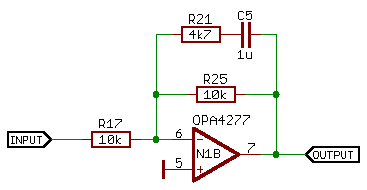
\includegraphics[width=\columnwidth]{graphics/60-hv-amp-dewhitening.pdf}
  \caption[Active inverting dewhitening circuit]{Active inverting dewhitening circuit. This filter uses an inverting op-amp with parallel feedback resistors to achieve the desired frequency response. At low frequencies, the capacitor's impedance is high and so the feedback path is dominated by the impedance of the \SI{10}{\kilo\ohm} resistor and the gain is \num{1}. At high frequencies the capacitor produces very impedance and the feedback path's impedance is the equivalent resistance of the parallel \SI{4.7}{\kilo\ohm} and \SI{10}{\kilo\ohm} resistors and the gain is then $\frac{\SI{10}{\kilo\ohm}}{\SI{3.2}{\kilo\ohm}} \approx \SI{-10}{\deci\bel}$.}
  \label{fig:hv-amp-dewhitening-circuit}
\end{figure}

\begin{figure}
  \centering
  \includegraphics[width=\columnwidth]{graphics/generated/from-python/60-hv-amp-dewhitening-sims.pdf}
  \caption[Simulated dewhitening filter frequency response]{Frequency response of the dewhitening filters simulated with \gls{LISO}. Each dewhitening filter provides \SI{-10}{\deci\bel} gain at high frequencies and so the combined pair produces an overall high frequency gain of $\SI{-20}{\deci\bel} \approx \num{e-1}$.}
  \label{fig:hv-amp-dewhitening-sims}
\end{figure}

\subsubsection{Digital switching electronics}
A series of digital outputs from \gls{CDS} can be used to control the \gls{HV} amplifier's dewhitening filters. The Contec DO-32L-PE output card provides a 32 channel binary switch with an equivalent schematic shown in the left side of Figure\,\ref{fig:hv-amp-sigital-switching}. The control signal from \gls{CDS} for a particular output is inverted and attaches to the negative input of an optocoupler, which acts as a relay without an electrical connection between the input and output. The positive input is attached to a voltage supply such that a digital output of \num{1} results in a closed circuit once inverted. An output of \num{0} is inverted to \num{1} and so there is no potential difference to close the optocoupler's circuit. The optocoupler's output in turn connects to the base of a transistor which controls current flow between the collector and emitter.

\begin{figure}
  \centering
  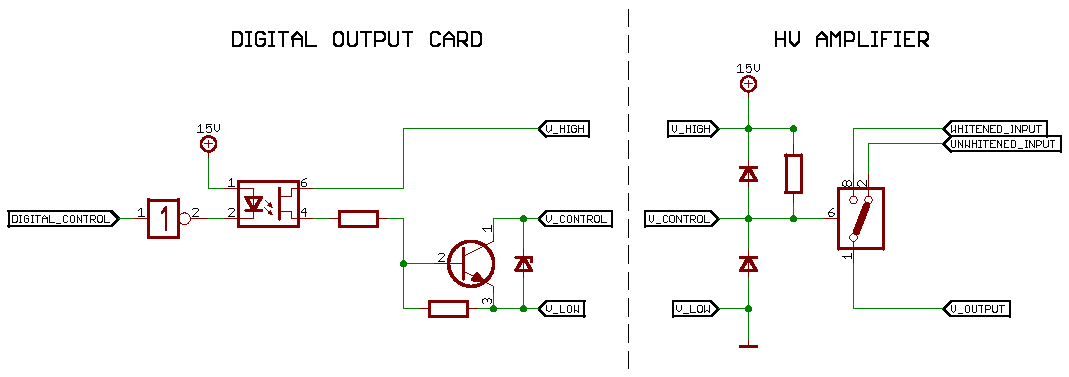
\includegraphics[width=\columnwidth]{graphics/60-hv-amp-digital-switching.pdf}
  \caption[Digital signalling between the control and data acquisition system and a channel within the high voltage amplifier]{\label{fig:hv-amp-sigital-switching}Digital signalling between \gls{CDS} and a channel within the \gls{HV} amplifier. The digital control signal operates an optocoupler which allows current to flow from the $V_{\text{HIGH}}$ voltage reference to a transistor which operates the analogue control signal $V_{\text{CONTROL}}$. This signal is used by the \gls{CMOS} switch in the \gls{HV} amplifier to select either the dewhitened or non-dewhitened signals.}
\end{figure}

The analogue input to the \gls{HV} amplifier for a particular channel is split into two with one passed through the dewhitening filter and the other unperturbed. These two signals form the poles of a \emph{complementary metal-oxide semiconductor} (\gls{CMOS}) switch, chosen for its switching speed, controlled by the digital signal which connects to one of the digital outputs of the \gls{CDS} card via a shielded transmission line. Due to the operation of the digital output card the dewhitening filter control signal $V_{\text{CONTROL}}$ must nominally be $V_{\text{HIGH}}$ which is achieved through the use of a pull-up resistor. When dewhitening is desired, an output of \num{1} at the optocoupler results in a low-resistance path between the control signal and ground and so the control signal within the amplifier becomes $V_{\text{LOW}}$. A truth table is shown in Table\,\ref{tab:digital-dewhitening-truth-table}.

\begin{table}
  \centering
  {\renewcommand{\arraystretch}{1.2} % for extra vertical spacing between rows
    \begin{tabular}{c|c|c}
      \textbf{\gls{CDS} software logic level} & \textbf{$V_{\text{CONTROL}}$} & \textbf{Dewhitening status} \\
      \hline
      0 & $V_{\text{HIGH}}$ & On \\
      1 & $V_{\text{LOW}}$ & Off
    \end{tabular}
  }
  \caption[Truth table for digital switching of dewhitening filters in the high voltage amplifier]{\label{tab:digital-dewhitening-truth-table}Truth table for digital switching of dewhitening filters in the \gls{HV} amplifier, showing the effect that a software logic level in \gls{CDS} has on the dewhitening of the input signal for a particular channel in the \gls{HV} amplifier.}
\end{table}

The electronics shown in Figure\,\ref{fig:hv-amp-sigital-switching} are for a single dewhitener. This configuration must be repeated twice for each of the amplifier's channels to control each of the dewhitening filters.

\subsection{Choice of high voltage op-amp}
Due to the nature of the load the amplifier does not need to drive a significant current, but the voltage noise it produces must be significantly lower than the displacement requirement for the experiment in order for it not to limit its sensitivity. The lowest noise high voltage amplifier integrated circuits available tend to be \gls{MOSFET}-type op-amps. The choice of device tends to be motivated by the bandwidth, maximum output voltage and noise of each particular model.

The \emph{gain-bandwidth product} specifies an op-amp's open-loop gain as a function of the bandwidth it is able to provide it over, and this figure is derived from the speed at which the op-amp's output is able to react to a change in its input (its \emph{slew rate}). The full output voltage is not provided at the unity gain frequency and so a more useful figure of merit is the bandwidth over which the maximum output can be provided. For the \SSMEXPT{} it is expected that radiation pressure and thermal noise will require fast corrections in the \SI{}{\kilo\hertz} range, and to avoid becoming limited by the device's slew rate at higher frequencies (which appears as phase lag on a plot of the frequency response) it is reasonable to require a bandwidth of at least \SI{20}{\kilo\hertz}.

The required \gls{DC} op-amp gain should be known ahead of time in order to fully estimate the effect an op-amp's noise will have on the experiment. The maximum \gls{CDS} input voltage is \SI{\pm10}{\volt} and so to achieve the maximum output voltage requirement when the \gls{CDS} voltage is maximum, thus giving the greatest dynamic range, the op-amp's gain should be set to around \num{40}. From this we can estimate the output noise of some op-amps and determine the Johnson-Nyquist noise (see Section\,\ref{sec:johnson-nyquist-noise}) contribution of the resistors that define the op-amp's \gls{DC} gain.

Table\,\ref{tab:hv-op-amp-comparison} shows the aforementioned parameters for some popular op-amp models. The models shown have sufficient output voltage and identical input noise. The PA89's bandwidth is limited and the full output voltage is not available beyond \SI{7}{\kilo\hertz}, whilst the quiescent power in the PA94 and PA98 is high enough to warrant challenging heat sink requirements. In this case the optimal choice of op-amp is the PA95, for which only a passive heat sink will be required.

\begin{table}
  \centering
  \begin{tabular}{r|c|c|c|c}
    & \textbf{PA89} & \textbf{PA94} & \textbf{PA95} & \textbf{PA98} \\
    \hline
    \textbf{Maximum output} & \SI{1140}{\volt} & \multicolumn{2}{c}{\SI{900}{\volt}} & \SI{450}{\volt} \\
    \textbf{Bandwidth @ \SI{400}{\volt} output} & \SI{7}{\kilo\hertz} & \SI{90}{\kilo\hertz} & \SI{30}{\kilo\hertz} & \SI{60}{\kilo\hertz} \\
    \textbf{Input noise @ \SI{100}{\hertz}} & \multicolumn{4}{c}{\SI{6}{\nano\volt\per\sqrthz}} \\
    \textbf{Quiescent power @ \SI{\pm400}{\volt}} & \SI{3.8}{\watt} & \SI{14.1}{\watt} & \SI{1.3}{\watt} & \SI{17.5}{\watt}
  \end{tabular}
  \caption[Performance specifications for various high voltage operational amplifiers]{\label{tab:hv-op-amp-comparison}Performance specifications for various \gls{HV} op-amps. All of the models listed are manufactured by Apex and the values have been obtained from their respective data sheets. The PA95 was selected due to its low quiescent power for the desired voltage range, which in turn eases the requirement for heat sinking, and the bandwidth is sufficient for the \SSMEXPT{}.}
\end{table}

\subsection{Amplifier signal path}
The amplifier signal path is shown for a single channel in Figure\,\ref{fig:hv-amp-signal-path}. The differential inputs IN+ and IN- are converted to a single-ended signal which is then passed through the two dewhitening stages controlled by digital switches. The signal is then split into two parts, with one part being inverted, before they are input to the PA95 power op-amps. The inputs are clamped together by diodes to ensure that the difference is less than \SI{0.7}{\volt}. This is to prevent the expensive op-amps from damage caused by overvoltage at the inputs, and does not limit the bandwidth or dynamic range in this application. A \SI{1}{\percent} voltage divider at each of the differential outputs provides a signal that is within the input range of \gls{CDS} for the purpose of output monitoring. This provides a readback channel for the controller in order to assist with the calibration of the device.

\begin{figure}
  \centering
  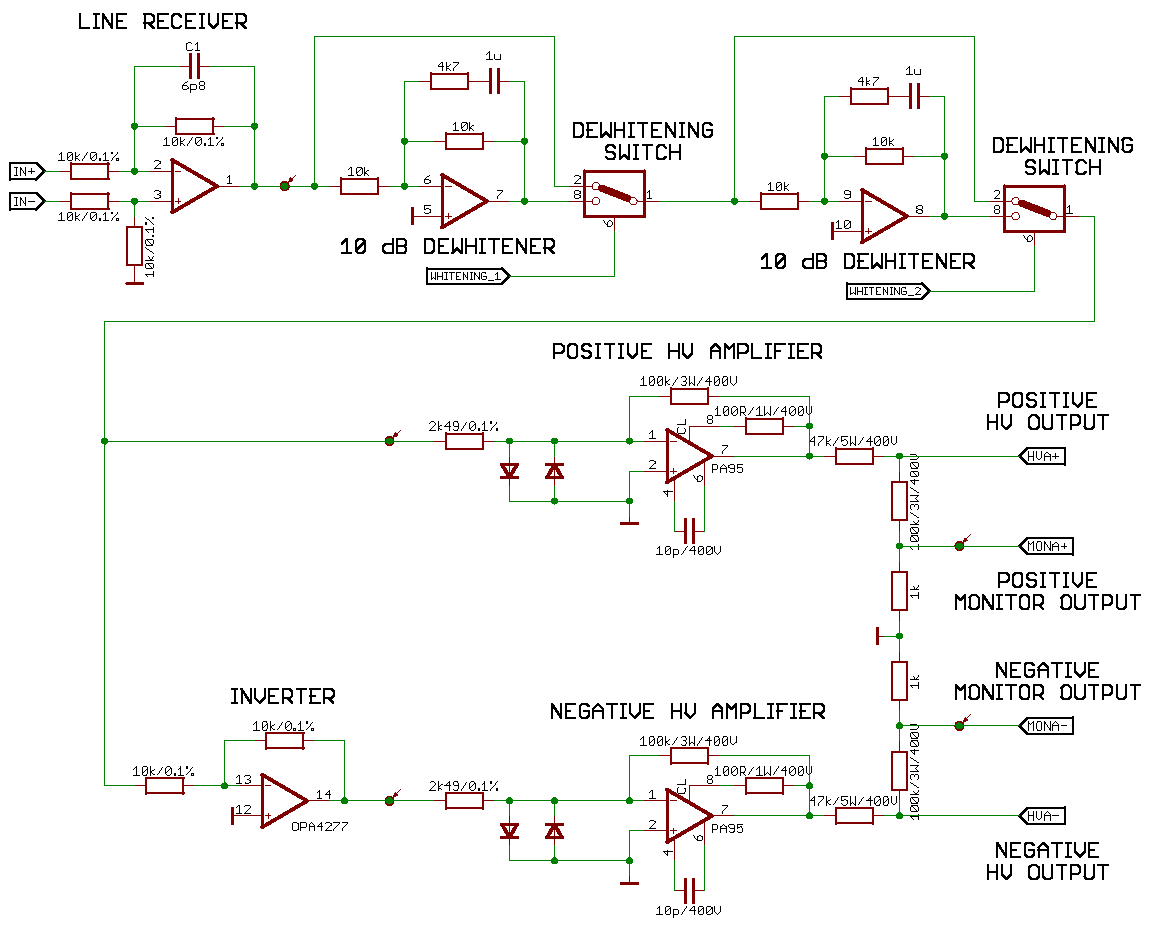
\includegraphics[width=\columnwidth]{graphics/60-hv-amp-signal-path.pdf}
  \caption[High voltage amplifier signal schematic]{\label{fig:hv-amp-signal-path}Schematic of a single high voltage amplifier channel. The input from \gls{CDS} is differentially received, dewhitened and then split into differential outputs that are amplified by PA95 op-amps. A pickoff reads \SI{1}{\percent} of the output voltage for the purposes of calibration.}
\end{figure}

\subsection{Practical and safety features}
As the \gls{HV} amplifier handles potentially lethal current and voltage, a number of additional features beyond the signal circuitry are present.

\subsubsection{Current limiting}
At the output of each \gls{HV} rail there are \SI{47}{\kilo\ohm} resistors which passively limit the current on each rail to around \SI{10}{\milli\ampere}. This operates in addition to an active current limit set via a \SI{100}{\ohm} witness resistor between two pins of each PA95 op-amp. The current limit does not impact the driving of capacitive loads, but ensures that the current produced by the \gls{HV} amplifier is not lethal.

\subsubsection{Soft-start}
Capacitors are present upon the \gls{HV} supply lines to filter \gls{AC} noise, and these must be charged when the device is switched on. Normally these capacitors would present very little impedance to the power supplies and so a large initial current would be drawn, potentially damaging components in its path. The simplest technique to prevent this from happening would be to put resistors in the path of the power supplies, but resistors that would charge the capacitors at a safe rate in a short time would also dissipate a lot of power and require heat sinking. Instead, we use a \emph{soft-start} mechanism which controls the current flow during the charging of the capacitors. The \gls{HV} amplifier's on-off switch operates some optocouplers which allow current to flow into the circuit. Initially, when the circuit's \gls{HV} capacitors are discharged the current on each \gls{HV} rail is limited by the parallel \SI{5}{\kilo\ohm} resistors. A \SI{2.5}{\percent} pick-off from each \gls{HV} rail is compared to a reference \SI{5}{\volt} voltage at an op-amp, the output of which operates a second optocoupler on each rail. When the voltage surpasses \SI{200}{\volt} the power the \SI{5}{\kilo\ohm} resistors dissipate is \SI{8}{\watt}, which is near the reasonable limit for passively cooled resistors. At this point, the capacitors are almost fully charged and the pick-off voltage surpasses the \SI{5}{\volt} reference, and so the op-amp's output operates the optocoupler to open up a low-resistance path that bypasses the \SI{5}{\kilo\ohm} resistors and prevents them from overheating. This is shown in Figure\,\ref{fig:hv-amp-soft-start}.

\begin{figure}
  \centering
  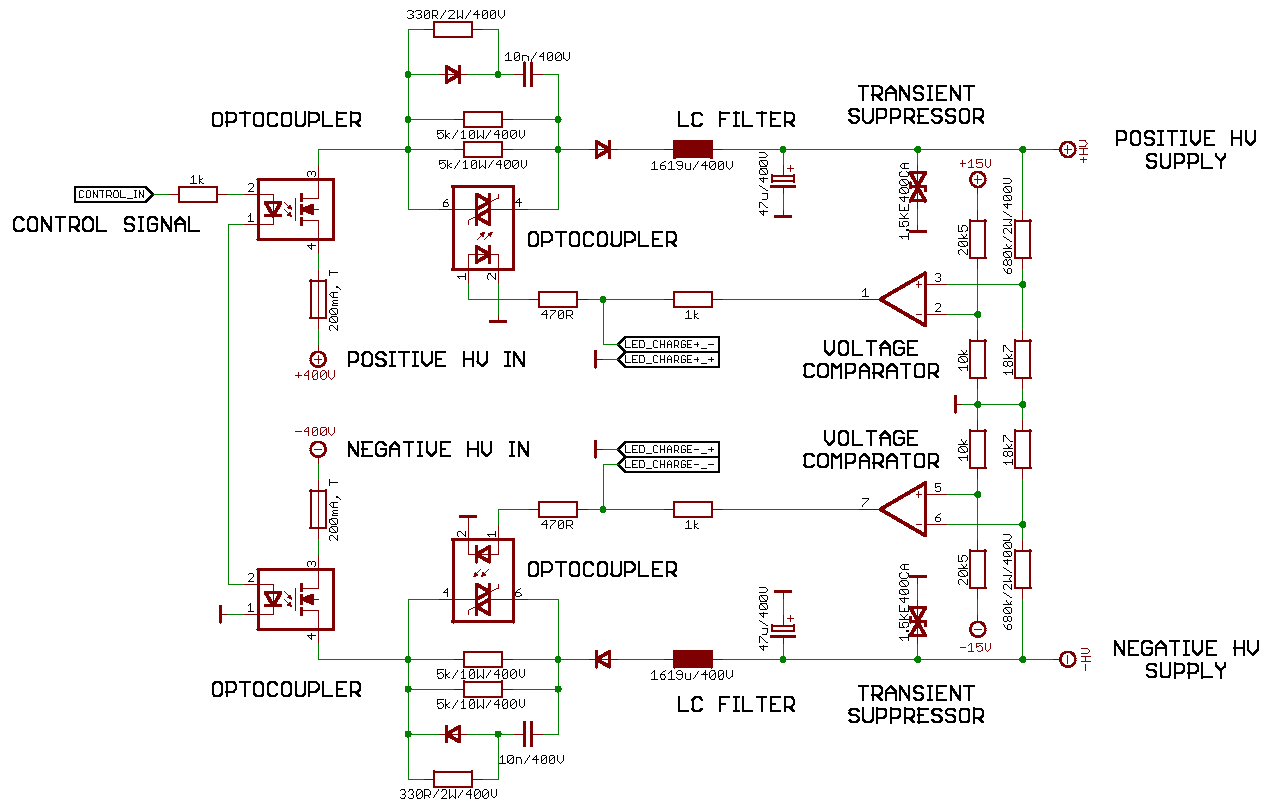
\includegraphics[width=\columnwidth]{graphics/60-hv-amp-soft-start.pdf}
  \caption[High voltage amplifier soft-start schematic]{\label{fig:hv-amp-soft-start}Soft-start mechanism to prevent excessive power supply current draw. This design is based on one the soft-start mechanism for a device produced for the \AEIPROTOTYPE{} by Andreas Weidner. The leftmost optocouplers control whether current is allowed to flow from the power supplies given a control signal from an on-off switch on the enclosure. After the electronics are switched on, the current flow is initially limited by two \SI{5}{\kilo\ohm} resistors. Any \gls{AC} signal content is filtered by the presence of a \SI{1.6}{\milli\farad} choke. A \SI{2.5}{\percent} pick-off from each \gls{HV} rail is compared to a \SI{\pm5}{\volt} reference, with the resulting difference fed back to a second pair of optocouplers which gradually open up a low-resistance path on each supply rail. Without these optocouplers, the power the \SI{5}{\kilo\ohm} resistors would need to dissipate would be considerable at maximum voltage. As the supply voltage increases beyond around \SI{200}{\volt}, the resistance through the optocoupler is reduced far below the \SI{5}{\kilo\ohm} resistors and so the power dissipated in the resistors is negligible.}
\end{figure}

\subsubsection{Pressure and temperature interlock}
The breakdown voltage of the plate capacitors as a function of pressure, given by Paschen's Law, has a minimum in the region of \SI{e-1}{\milli\bar} to \SI{e1}{\milli\bar} depending on the separation and geometry of the anode and cathode, as shown in Figure\,\ref{fig:esd-paschen}. In addition, related effects such as surface tracking can lead to arcing at voltages above \SI{50}{\volt} in low vacuum.

Although the use of high voltage plate capacitors is in general safe at both atmospheric pressure and high vacuum, the act of pumping gas out of the vacuum system necessarily passes through pressures at which arcing can occur. To prevent the possibility of arcing, a cut-off function is present within the circuit to prevent high voltage output unless a control signal is supplied (see Figure\,\ref{fig:hv-amp-interlock}). This signal will be produced by \gls{CDS} derived from a separate pressure monitor. Additionally, as a temperature fail-safe for the amplifier components, temperature sensors are present within the enclosure which operate threshold switches able to remove the supply current via the same mechanism as the pressure interlock. The outputs from each interlock are sent to an AND gate. Only if both the pressure and temperature switches are switched on will the control signal used to operate the \gls{HV} supplies switch on. The interlock circuit is shown in Figure\,\ref{fig:hv-amp-interlock}.
% pressure vs voltage claim from speedmeter labbook, at https://arran.physics.gla.ac.uk/wp/speedmeter/2015/01/30/esd-hv-amplifier-pressure-cutoff/

\begin{figure}
  \centering
  \includegraphics[width=\columnwidth]{graphics/generated/from-python/60-esd-paschen.pdf}
  \caption[Minimum breakdown voltage between the two plates of the electrostatic drive for different separations]{\label{fig:esd-paschen}The minimum breakdown voltage between the two plates of the \gls{ESD} for different separations. This is calculated using Paschen's Law, assuming nitrogen gas and a flat plate geometry. The real effect is a lot more complicated than this model, but the steep slope at lower pressures shown here indicates that the voltage created by the \gls{HV} amplifier for the \gls{ESD} experiment will avoid problems associated with arcing as long as it is operated at atmosphere or high vacuum.}
\end{figure}

\begin{figure}
  \centering
  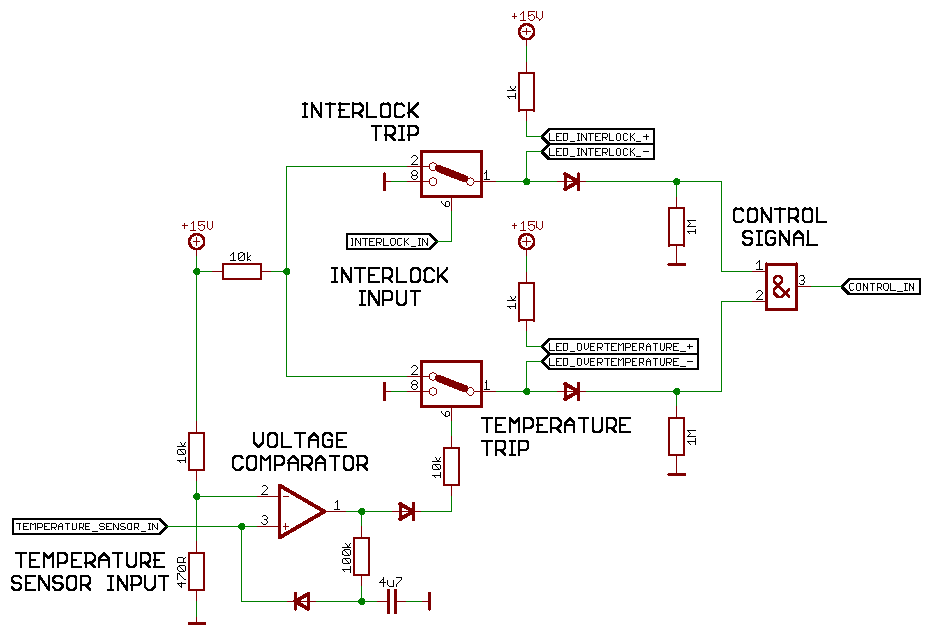
\includegraphics[width=\columnwidth]{graphics/60-hv-amp-interlock.pdf}
  \caption[High voltage amplifier interlock schematic]{\label{fig:hv-amp-interlock}Pressure and temperature interlock circuit. The digital interlock signal from \gls{CDS} operates one switch and the output from a temperature sensor threshold switch operates another. Only if both switches output \SI{15}{\volt} will the control signal used to operate the \gls{HV} supplies switch on.}
\end{figure}

\subsection{Transfer functions and noise measurements}
Transfer functions for the \gls{HV} amplifier can be measured by injecting a known signal into one channel and measuring the corresponding output. The monitor output provides a means of measuring \SI{1}{\percent} of the full \gls{HV} output with a signal that is within the input range of \gls{CDS}.

\subsubsection{Swept sine response of each channel}
Figure\,\ref{fig:hv-amp-dewhitened-tfs} shows the \emph{swept sine} response, calculated by injecting a sine wave at a given frequency, measuring the output signal and dividing it by the injection. These measurements were made without the digital dewhitening switches engaged such that they provide \SI{20}{\deci\bel} of low-pass filtering. The figure shows the response expected from the predictions made by \gls{LISO} shown in Figure\,\ref{fig:hv-amp-dewhitening-sims}.

\begin{figure}
  \centering
  \includegraphics[width=\columnwidth]{graphics/generated/from-python/60-hv-amp-dewhitened-tfs.pdf}
  \caption[Frequency response of the high voltage amplifier's channels with dewhitening enabled]{Second amplifier transfer functions with dewhitening enabled. The expected performance of the dewhitening filter from theory is shown in \checkme{purple} alongside the transfer functions of each channel. The curves agree closely, showing that the implemented filter operates as expected. The mismatch at high frequency is caused by the anti-aliasing filters implemented in \gls{CDS}, which aggressively filter signals above a few \SI{}{\kilo\hertz}.}
  \label{fig:hv-amp-dewhitened-tfs}
\end{figure}

\subsubsection{Response with and without dewhitening}
Figure\,\ref{fig:hv-amp-channel-one-tfs} shows swept sine measurements of the first channel with the dewhitening filters in various states: both on, the first on and the second off, the first off and the second on, and both off. The measurements match predictions and the response with both dewhiteners off is flat as intended across the measurement band.

\begin{figure}
  \centering
  \includegraphics[width=\columnwidth]{graphics/generated/from-python/60-hv-amp-channel-one-tfs.pdf}
  \caption[Transfer functions of the high voltage amplifier input to monitor output with the dewhiteners on and off]{Transfer functions of the high voltage amplifier input to monitor output with the dewhitening filters on and off. The monitor output is a \SI{1}{\percent} pick-off from the main \gls{HV} output, and so the gain is \num{0.4} instead of \num{40}. The curves simulated with \gls{LISO} agree exactly with the measurements within the bandwidth of \gls{CDS}, and beyond around \SI{3}{\kilo\hertz} the transfer functions are suppressed by the anti-aliasing filters on \gls{CDS}'s \glspl{ADC}.}
  \label{fig:hv-amp-channel-one-tfs}
\end{figure}

\subsubsection{Coherence between channels}
The channels should be isolated from one another such that a signal injected at one input does not appear at the output of another. Power supply filtering is implemented using capacitors, inductors and diodes such that there should be minimal cross-coupling between the channels. Figure\,\ref{fig:hv-amp-coherence} shows the coherence for each channel to each other channel, measuring whether the output signal has the same phase angle as the input signal. Coherence of \num{1} indicates that there is causal coupling between the two channels, whereas coherence less than around \num{0.5} is expected from statistical random noise processes. This confirms that a high level of isolation between channels is achieved.

\begin{figure}
  \centering
  \includegraphics[width=\columnwidth]{graphics/generated/from-python/60-hv-amp-coherence.pdf}
  \caption[High voltage amplifier cross-channel coherence]{\gls{HV} amplifier cross-channel normalised coherence. A swept sine was injected into each channel in turn whilst measurements of the output phase were made on all four channels. In each case, only the channel with the injection has coherence of \num{1}, while other channels only show the effect from noise.}
  \label{fig:hv-amp-coherence}
\end{figure}

\subsubsection{Output noise}
The noise at the output of the \gls{HV} amplifier is shown in Figure\,\ref{fig:hv-amp-output-noise}. This was calculated via the \gls{HV} amplifier's monitor, with the measurements projected into effective \gls{HV} noise by multiplying the signal by the inverse of the monitor pick-off fraction, \num{100}. To measure the noise at frequencies comparable to the \SSMEXPT{}'s cavity bandwidth a Stanford Research SR785 spectrum analyser was used; as shown in Figure\,\ref{fig:aa-ai-filter-tfs} the anti-imaging filters significantly reduce the output from \gls{CDS} above \SI{9}{\kilo\hertz} and so they are not practical for this measurement.

The following measurements were made:
\begin{itemize}
  \item the \gls{HV} amplifier's output noise when it is disconnected from \gls{CDS} and has no input signal;
  \item the \gls{HV} amplifier's output noise when it is connected to the \gls{CDS} \glspl{DAC} with an input signal equivalent to maximum \gls{HV} output;
  \item the spectrum analyser noise floor with a \SI{50}{\ohm} load.
\end{itemize}
Each of the spectral densities shown were produced using Fourier transforms of the time domain signal (see Appendix\,\ref{sec:fourier-transform}), and to avoid windowing effects as discussed in Appendix\,\ref{sec:windowing} the measurements were made with averages across three bands: \SI{250}{\milli\hertz} to \SI{200}{\hertz} (\num{16} averages), \SI{4}{\hertz} to \SI{3.2}{\kilo\hertz} (\num{64} averages) and \SI{128}{\hertz} to \SI{102.4}{\kilo\hertz} (\num{1024} averages). The measured output noise is above the input noise of the spectrum analyser.

The projected \gls{HV} noise is different in the case of zero or full \gls{DC} output not because of an input voltage dependency but rather due to the inclusion of the \gls{CDS} \glspl{DAC} in the signal path in the latter case which contribute noise as discussed in Section,\ref{sec:adcs-and-dacs}.

\begin{figure}
  \centering
  \includegraphics[width=\columnwidth]{graphics/generated/from-python/60-hv-amp-output-noise.pdf}
  \caption[High voltage amplifier output noise]{\gls{HV} amplifier output noise. The noise of the amplifier was measured using the monitor output of the first channel and the noise shown has been corrected for the monitor pick-off fraction. The \checkme{green} curve shows the noise from the amplifier when the input is at maximum and includes the noise contribution from the \glspl{DAC} on \gls{CDS}. The \checkme{orange} curve shows the noise when \gls{CDS} is not connected. The noise floor of the spectrum analyser used to make these measurements is shown in \checkme{blue}.}
  \label{fig:hv-amp-output-noise}
\end{figure}

The effective displacement noise the \gls{HV} amplifier would produce on the \gls{ETM} suspensions can be calculated using a simple argument. At a frequency within the measurement band of the \SSMEXPT{}, \SI{100}{\hertz}, the projected voltage noise from the \gls{HV} amplifier is around \SI{30}{\micro\volt\per\sqrthz}. We know that the force depends on the square of the potential difference, and rearranging Equation\,\ref{eq:esd-force},
\begin{equation}
  \frac{F \left( \SI{750}{\volt} \right)}{\left( \SI{750}{\volt} \right)^2} = \frac{F \left( \SI{30}{\micro\volt} \right)}{\left( \SI{30}{\micro\volt} \right)^2},
\end{equation}
we can calculate the force noise on the \gls{ETM} at \SI{100}{\hertz} to be of the order $F \left( \SI{30}{\micro\volt} \right) = \SI{e-21}{\newton\per\sqrthz}$. The displacement noise is then, using Figure\,\ref{fig:ssm-etm-disp-vs-esd-force}, around \SI{e-26}{\meter\per\sqrthz}. This is eight orders of magnitude below the requirement shown in Figure\,\ref{fig:noise-budget} and shows that electronic noise from the \gls{HV} amplifier will not present a problem to the sensitivity of the experiment.

% No data yet
% \section{Experimental test of the electrostatic drive}
% To set requirements on the positioning of the plates, and to build and test the infrastructure for the operation of the \glspl{ESD}, this chapter introduces the design for an experiment to test the new \gls{ESD} design.
% 
% \begin{table}
%   \centering
%   \begin{tabular}{ll}
%     \textbf{Parameter}   & \textbf{Value} \\
%     Mirror diameter      & \SI{30}{\milli\meter} \\
%     Mirror thickness     & \SI{6}{\milli\meter} \\
%     Single plate width   & \SI{30}{\milli\meter} \\
%     Single plate length  & \SI{50}{\milli\meter} \\
%     Nominal plate separation & \SI{40}{\milli\meter} \\
%   \end{tabular}
%   \caption[Plate capacitor and optic parameters for the experiment to test the electrostatic drives for the \SSM{}]{\label{tab:esd-expt-parameters}Plate capacitor and optic parameters for the experiment to test the electrostatic drives for the \SSM{}.}
% \end{table}
% 
% Although the \gls{ESD}, and indeed the \SSM{} experiment, primarily require corrections at lower frequencies where seismic noise is dominant, it is beneficial to utilise an amplifier which can provide actuation up to many tens, if not hundreds, of \SI{}{\kilo\hertz}. This facilitates a transfer function which is flat across the vast majority of each experiment's measurement band, avoiding the roll-off at high frequencies due to the integrated circuits utilised within the high voltage amplifier. A flat transfer function makes the calibration of the actuator plant as part of the overall experiment as simple as possible. Another benefit of having a high bandwidth amplifier is the possibility to use it for common mode control loops, where laser frequency stabilisation can be split between feedback to the laser's piezoelectric transducer and actuators on the test masses.
% 
% The key component of a high bandwidth amplifier is the power op-amp. This class of op-amps typically utilises a \gls{MOSFET} design, and can provide high voltage output given a low voltage input. As an example, the Apex PA95 op-amps used in Advanced LIGO's \glspl{ESD} provide up to \SI{900}{\volt} output up to a frequency of around \SI{15}{\kilo\hertz}, and up to \SI{50}{\volt} at \SI{250}{\kilo\hertz}. The PA98 op-amp, also from Apex, provides an output of \SI{450}{\volt} nominally up to \SI{60}{\kilo\hertz}, potentially up to \SI{500}{\kilo\hertz} for a low capacitive load. For the purposes of this experiment, the choice was made to use the PA98 op-amp to provide the ability to study the effect of the actuator across a very wide bandwidth. To this end, an amplifier circuit utilising the PA98 was built based on a design used for the \AEIPROTOTYPE{}. This design provides up to \SI{\pm350}{\volt} output, and originates from a single-ended, \SI{350}{\volt} amplifier design where the PA98 is especially suited. Two notable modifications have been made, with a view to safety.
% 
% % claim about voltage output of PA95 comes from figure ``Power Response'' on p3 of PA95 datasheet (https://www.apexanalog.com/resources/products/pa95u.pdf)
% % claim about voltage output of PA98 comes from figure 8: ``power Response'' on p7 of PA98 datasheet (https://www.apexanalog.com/resources/products/pa98u.pdf)

\section{Outlook}
Parallel plate capacitor \glspl{ESD} provide a low noise alternative to voice coil actuators for the control of suspended test masses, and it is intended for \glspl{ESD} to be used as the high frequency actuators in the \SSMEXPT{}. In order to provide actuation at the required level, an \gls{HV} signal must be supplied to each \gls{ESD}. The technical design of an \gls{HV} amplifier was presented with the intention to provide actuation at the required magnitude and with low enough noise to meet the experiment's sensitivity requirement, and measurements of the implemented apparatus verify that this is the case.